\documentclass[12pt]{article}
\setlength\parindent{0pt}
\usepackage{fullpage}
\usepackage{amsmath}
\usepackage{graphicx}
\usepackage[margin=0.5in]{geometry}
\setlength{\parskip}{4mm}
\def\LL{\left\langle}   % left angle bracket
\def\RR{\right\rangle}  % right angle bracket
\def\LP{\left(}         % left parenthesis
\def\RP{\right)}        % right parenthesis
\def\LB{\left\{}        % left curly bracket
\def\RB{\right\}}       % right curly bracket
\def\PAR#1#2{ {{\partial #1}\over{\partial #2}} }
\def\PARTWO#1#2{ {{\partial^2 #1}\over{\partial #2}^2} }
\def\PARTWOMIX#1#2#3{ {{\partial^2 #1}\over{\partial #2 \partial #3}} }
\newcommand{\BE}{\begin{displaymath}}
\newcommand{\EE}{\end{displaymath}}
\newcommand{\BNE}{\begin{equation}}
\newcommand{\ENE}{\end{equation}}
\newcommand{\BEA}{\begin{eqnarray}}
\newcommand{\EEA}{\nonumber\end{eqnarray}}
\newcommand{\EL}{\nonumber\\}
\newcommand{\la}[1]{\label{#1}}
\newcommand{\ie}{{\em i.e.\ }}
\newcommand{\eg}{{\em e.\,g.\ }}
\newcommand{\cf}{cf.\ }
\newcommand{\etc}{etc.\ }
\newcommand{\Tr}{{\rm tr}}
\newcommand{\etal}{{\it et al.}}
\newcommand{\OL}[1]{\overline{#1}\ } % overline
\newcommand{\OLL}[1]{\overline{\overline{#1}}\ } % double overline
\newcommand{\OON}{\frac{1}{N}} % "one over N"
\newcommand{\OOX}[1]{\frac{1}{#1}} % "one over X"

\pagenumbering{gobble}

\begin{document}
\Large
\centerline{\sc{Recitation Questions}}
\normalsize
\centerline{\sc{24 April}}


 A bucket of mass $m$ hangs from a string wound around a pulley 
(a solid cylinder) with mass $M$ and radius $r$. When the bucket is
released, it falls, unwinding the string.

\begin{enumerate}

\item Draw force diagrams for the bucket and the pulley. Note that since the pulley rotates, you will need
to draw an extended force diagram for it, drawing the object and labeling where each force acts.

\vspace{3in}

\item In terms of the forces in your force diagrams, write an expression for the net torque on the pulley.

\vspace{1in}

\item Write down Newton's laws of motion -- $\sum \vec F = m \vec a$ for translation, and $\sum \tau = I \alpha$
-- for each object. (One object moves, and the other turns...)

\vspace{2in}


\newpage

\item What is the relationship between the angular acceleration $\alpha$ of the pulley and the linear acceleration
$a$ of the bucket? (The answer may be different depending on how you have drawn your pictures and your choice of
coordinate system.)

\vspace{1in}

\item Calculate the acceleration of the bucket in terms of $m$ and $M$.

\vspace{4in}

\item Suppose that the pulley were a hollow cylinder with the same mass. How would this acceleration change?

\newpage
\end{enumerate}

A simplified model of a car or truck can be thought of as shown below. Consider
the body of the vehicle to be a uniform plate of mass $M$, supported by the
normal force of two axles, each located a distance $L/6$ from each end.
The engine, also of mass $M$, is located a distance $L/6$ from the front. (Don't worry about 
distinguishing the left wheels from the right ones; you can treat ``front wheels'' and ``back wheels''
as single forces.) Note that the car is pointed to the left here (since the engine is in the front).

\begin{center}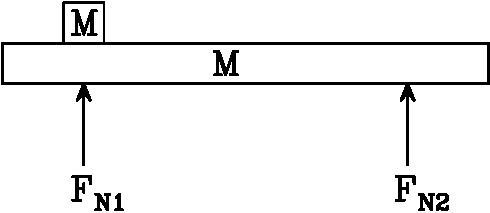
\includegraphics[width=0.5\textwidth]{car-crop.pdf}\end{center}
\begin{enumerate}

\item Without doing any mathematics, do you expect the normal force from the front wheels 
or from the rear wheels to be larger? Why?

\vspace{1in}

\item Draw an extended force diagram for the vehicle.

\newpage

\item Calculate the normal forces $F_{N1}$ and $F_{N2}$ exerted by each axle.

\vspace{3in}

\item Suppose that the coefficient of friction between the wheels and the ground is $\mu_s$. What is the maximum
traction force that the car can apply if it is front wheel drive? (Most passenger sedans, like my Toyota Yaris,
are front wheel drive.)

\vspace{3.5in}

\item What is the maximum traction force that the car can apply if it is rear-wheel drive? (Most pickup trucks that
only have two driven wheels are rear-wheel drive.)

\vspace{3.5in}

\item Often people with two-wheel-drive pickup trucks will pile snow in the back of the truck during the Syracuse winter.
Why do they do this?

As a hint, the thing that determines whether you will get stuck or not in slippery conditions is often the ratio between
the traction force and the total mass of the vehicle.



\end{enumerate}
\newpage
\Large
\centerline{\sc{Recitation Questions}}
\normalsize
\centerline{\sc{26 April}}

Consider a Ping-Pong ball resting on a smooth table. (Since this is a hollow shell, its moment of inertia is 
$I=\frac{2}{3}mr^2$.) The coefficient of static friction between the ball and the table is $\mu_s$, 
the coefficient of kinetic friction is $\mu_k$, and the 
ball has a mass $m$ and radius $r$.

A gentle breeze begins to blow, exerting a force $F_w$ on the ball that is much less than $mg$. (Since this force is spread out uniformly over the ball,
you may treat it as acting at the center of the ball.)

\begin{enumerate}

\item Draw an extended force diagram for the ball.

\vspace{4in}

\newpage

\item How large will the frictional force between the ball and the table be? (Note that $\mu_s F_N$ is only the 
{\it maximum} force of static friction.)

\vspace{3in}

\item Now, suppose that a gust of wind strikes the ball, so that $F_w$ becomes larger. How large can the wind force
be so that the ball rolls without slipping, instead of skidding?

\vspace{2in}

\item Suppose that the wind force is larger than this, so that the ball {\it skids}. Calculate both its angular
acceleration and its translational acceleration.
\end{enumerate}

\newpage

\begin{minipage}{0.5\textwidth}
A table has a mass $m$, and its height is $2/3$ of its width. The legs of the table are very light; all of the mass is in the top.
The legs of the table are located at the ends, and a rope is tied to one side; a tension $T$ is applied to the rope. Assume that the coefficient of friction between
the legs and the ground is very large, so that the table does not slide.
\end{minipage}
\begin{minipage}{0.5\textwidth}
\begin{center}
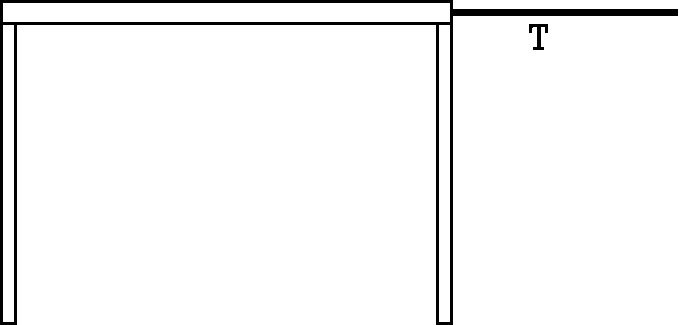
\includegraphics[width=0.7\textwidth]{table-crop.pdf}
\end{center}
\end{minipage}

In this problem, you will calculate the required tension $T$ to tip the table.

\begin{enumerate}

\item Draw a force diagram for the table. Indicate your choice of pivot.

\newpage

\item What tension force $T$ is required to tip the table (so that the back legs come off the ground)?
(Hint: What is true about the normal forces on the table when it begins to tip?)

\vspace {4in}

\item What coefficient of static friction between the legs and the floor is
required so that the table tips, rather than sliding?

\end{enumerate}
 \end{document}
